\documentclass{article}
\title{\textbf{A C++ Concepts}}
\author{}
\date{} 

\UseRawInputEncoding
\usepackage{graphicx}
\usepackage{hyperref}
\hypersetup{
    colorlinks=true,
    linkcolor=blue,
    filecolor=magenta,      
    urlcolor=cyan,
}
 
\urlstyle{same}

% Code Coloring
\usepackage{listings}
\usepackage{color}

\definecolor{dkgreen}{rgb}{0,0.6,0}
\definecolor{gray}{rgb}{0.5,0.5,0.5}
\definecolor{mauve}{rgb}{0.58,0,0.82}
\lstset{frame=tb,
  language=C++,
  aboveskip=3mm,
  belowskip=3mm,
  showstringspaces=false,
  columns=flexible,
  basicstyle={\small\ttfamily},
  numbers=none,
  numberstyle=\tiny\color{gray},
  keywordstyle=\color{blue},
  commentstyle=\color{dkgreen},
  stringstyle=\color{mauve},
  breaklines=true,
  breakatwhitespace=true,
  tabsize=3
}

%Box Note
\usepackage{graphicx}
\usepackage{tcolorbox}
\tcbuselibrary{skins}
\usepackage{lipsum}
\definecolor{boxTitle}{HTML}{fff79a}
\definecolor{boxBackground}{HTML}{fffce0}
\definecolor{boxFrame}{HTML}{f1e2b8}

\tcbset{my box/.style={
    enhanced, fonttitle=\bfseries,
    colback=boxBackground, colframe=boxFrame,
    coltitle=black, colbacktitle=boxTitle,
    attach boxed title to top left={xshift=0.3cm,
                                    yshift*=-\tcboxedtitleheight/2},
    boxed title style={
      before upper=\hspace*{0.5cm}, % reserve space for the image
      overlay={
       \node at ([xshift=0.5cm]frame.west)
         {\includegraphics[scale=0.65]{bc-dodecaedre}};
      }
    }
  }
}

\newtcolorbox{mybox}[1][]{my box, #1}

\begin{document}
\textbf{Disclaimer}: This material is a study notes, so for any technical issues please contact me to resolve it periodically.

\begin{minipage}{\textwidth}
    \maketitle
\end{minipage}
\tableofcontents
\lstlistoflistings

\section{Tips and Tricks}
\subsection{Pointer V.s. references}
The references are only introduced in C++, and it refers to an \textbf{"alias"} name for a certain existing variable. it's not an actual memory location.\\
It differs from pointers that the pointers are actual address holders but reference are not, and references can't be null and should be assigned to value in declaration. 
A reference cannot be re-assigned, and must be assigned at initialization.

\lstinputlisting[language=C++, caption=Pointer V.s.  references]{cpp_code/basic/references-pointers}
\textbf{Observation}:\\
\begin{center}
  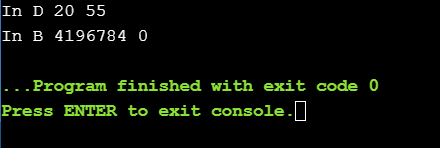
\includegraphics[scale=0.75]{./cpp_code/basic/sliceoff.PNG}
\end{center}

\textbf{Observation}:\\
\begin{center}
  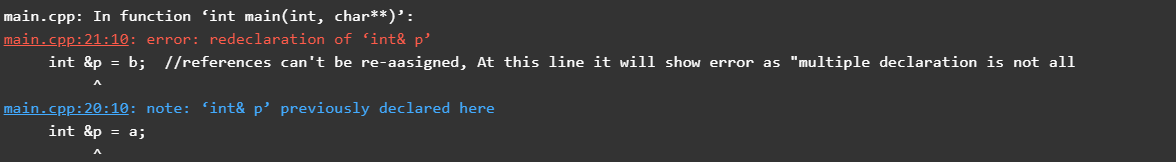
\includegraphics[scale=0.75]{./cpp_code/basic/refsvspointers.PNG}
\end{center}

\subsection{Forward declarations in C++}

\subsection{Object Slice off}
In C++, a Base class object can only be assigned to a Derived class object, but the other way is not possible.
Object slicing happens when a derived class object is assigned to a base class object, additional attributes of a derived class object are sliced off to form the base class object.

\lstinputlisting[language=C++, caption=Object Slice-off example]{cpp_code/basic/obj-sliceoff.cpp}

\subsection{C++ Constructors Types}
In C++ there are different types of constructors:
\begin{itemize}
  \item Default Constructor
  A default constructor is a contractor that takes no parameters, or one or all of its parameters has a default value

  For each class the default constructor is there, unless it's been explicitly deleted, and it can be deleted for any of the following reasons:
  \begin{itemize}
    \item 
  \end{itemize}

  \lstinputlisting[language=C++, caption=The Default constructors]{cpp_code/constuctors/the-default-constructor.cpp}


  \item Parameterized Constructor
  
  Please refer also to \ref{explicit_constructors} the explicit constructors

  \item Copy Constructor
  The copy constructor is the constructor which its parameters is an object from the same class, and it's purpose is to copy this object to a brand-new object. please also refer to \ref{shallow_copy} the shallow copying section.

  \lstinputlisting[language=C++, caption=The copy constructors]{cpp_code/constuctors/copy-constructor.cpp}


\end{itemize}

\subsubsection{The explicit constructors (the explicit specifier)} \label{explicit_constructors}
In C++ an implicit type conversion happens if a class have a constructor with at least one parameter. but the \textit{explicit} keyword is used to prevent that.
\lstinputlisting[language=C++, caption=The implicit type conversion]{cpp_code/basic/implicit-constuctors.cpp}

If we tagged a constructor as explicit, then an implicit conversion won't happen. so if you need to have it work, you need to call the constructor explicitly.
\lstinputlisting[language=C++, caption=The explicit construction]{cpp_code/basic/explicit-constuctors.cpp}

\subsection{C++ Objects Construction Order}
During the construction, the following construction order is been executed:

\begin{itemize}
  \item During Construction
  \begin{enumerate}
    \item Constructors of virtual base classes are executed, in the order that they appear in the initialization list.
    \item Constructors of non-virtual base classes are executed, in the declaration order.
    \item Constructors of class private members are executed in the declaration order (regardless of their order in the initialization list).
    \item The body of the constructor is executed.
  \end{enumerate}

  \item During Destruction
  \begin{enumerate}
    \item In a reverse order, the destructors of the derived classes will be called first, then the base classes destructors a reverse order to the initialization.
    \item The body of the destructor are called 
  \end{enumerate}
\end{itemize}
Let's have a simple example
\lstinputlisting[language=C++, caption=Object Construction Order]{cpp_code/constuctors/order-of-construction.cpp}

\subsection{The constructor V.s. the equal assignment operator}
In C++, you need to understand when exactly a constructor is called and on the other hand when the equal assignment operator is called, let's have the following example:

\lstinputlisting[language=C++, caption=Constructors V.s. equal operators]{cpp_code/basic/assignement-vs-construtors.cpp}

The point here is that the equal operator (=) will ONLY be called when we a have a constructed objects.

\subsection{Shallow Copying (THE RULE OF THREE)}
\label{shallow_copy}
When creating copies of arrays or objects one can make a deep copy or a shallow copy. A shallow copy can be made by simply copying the reference, but in deep copying you make it by copying every element of the object or an array to another location. let's have an example to understand:\\
In this example, we create normal two objects from the Point class, and when we copy the P2 = P1, P1 is copied to an independent copy to P2. then this is deep copying.
\lstinputlisting[language=C++, caption=Object Deep Copy]{cpp_code/basic/rule-of-three/shallow-vs-deep-objects.cpp}

What if we modified the Point class to have one member \textbf{"pointer"} variable.
\lstinputlisting[language=C++, caption=Object Shallow copy]{cpp_code/basic/rule-of-three/shallow-vs-deep-objects2.cpp}

As you can see that the pointer P is referring to the same value in both independent objects P1, and P2 !, and this is called \textit{"shallow copy"}; as in a shallow copy can be made by simply copying the reference\\
You might need to override this behavior by defining a copy constructor to allows make a new copy of the pointers in your class.

\lstinputlisting[language=C++, caption=Define copy constructor for deep copy]{cpp_code/basic/rule-of-three/shallow-vs-deep-objects3.cpp}

\subsubsection{Deep Copying needs the rule of three}
In C++, The rule of three and rule of five (in C++11) are rules of thumb for the building of exception-safe code and for formalizing rules on resource management. It accomplishes this by prescribing how the default members of a class should be used to accomplish this task in a systematic manner.\\

The rule of three/five says: 
If a class defines one (or more) of the following it should probably explicitly define all five (and of course a deep copying needs that).
\begin{itemize}
  \item destructor
  \item copy constructor
  \item copy assignment operator
  \item move constructor (C++ 11)
  \item move assignment operator (C++ 11)
\end{itemize}

\subsection{C++ Exception Class}
In C++ you can inherit the \textit{exception} class and define your own exceptions, but you need to be caution when passing this exception to a catch block, \textbf{You shouldn't catch an exception by value!.}\\
Let's see if we catch an exception by value:
\lstinputlisting[language=C++, caption=Catching excpetions by value]{./cpp_code/basic/exceptions/exception-problem.cpp}

The exception object is sliced off, and the message and code will not be available.

The solution to that is to catch the exception by reference. not by value.
\lstinputlisting[language=C++, caption=Catching excpetions by reference]{./cpp_code/basic/exceptions/exception-solution.cpp}

Note: always throw by value (don't throw by pointer) and catch by reference.\\

\subsubsection{difference between throw, and throw e}
If you are planning to re-throw the exception again you need to understand the difference between \textit{throw} and {throw e} within the catch context.\\

\lstinputlisting[language=C++, caption=Re-throw an exception]{./cpp_code/basic/exceptions/rethrow-exceptions.cpp}

\subsubsection{Stack Un-winding}
When you throw an exception from a function that doesn't have the catch clause, then this function will be destroyed from the stack, and the exception handler searches on the caller function for the exception handling, if it still doesn't exists, then it searches again for the caller in the call stack and this is called \textbf{stack unwinding}.\\
sometimes this can cause issues like memory leaks, let's have an example:

\lstinputlisting[language=C++, caption=Stack  Un-winding]{./cpp_code/basic/exceptions/stack-unwinding.cpp}

So how can we solve that ? Is by using RAII techniques!, Simply you can used smart pointer in this condition as one of RAII techniques.

\begin{mybox}[title={RAII - Mutex that locks itself!}]
From CppReference: \textbf{Resource Acquisition Is Initialization} or RAII, is a C++ programming technique which binds the life cycle of a resource that must be acquired before use \textbf{to the lifetime of an object.}\\
Which means if the object is gone the resource will be released and will be available for others to used.\\

\lstinputlisting[language=C++, caption=RAII - the lock that releases itself]{cpp_code/basic/exceptions/raii-mutex-unlocks-itself.cpp}

C++ 11 provide some new features for this purpose, like lock\_gurad, smart pointers, ... and so one. For more info: please visit \href{https://en.cppreference.com/w/cpp/language/raii}{this}
\end{mybox}
\subsubsection{Some tips of exception safety}
\begin{itemize}
  \item \textit{throw e}, will make a new instance of the exception call and throw it again.
  while \textit{throw} only will re-throw the current exception and to be catch in the next clause.
  \item Don't throw exceptions while objects construction failures, the object will be thrown away and the resources might not be released.
  Alternative: Use a flag to inform other members that construction failed
  \item Don't throw exceptions on the object destruction
  \item Don't throw exception in overloaded delete or delete[] operators, it might cause a memory leaks.
\end{itemize} 

\href{http://stroustrup.com/except.pdf}{You might have a look also at this resources: Exception Safety }


\subsection{The const safe member functions}
Normally we use the const keyword to keep the values unmodified, that's true and in C++ we use also to provide a const safe functions that are not allowed to modify the members of a certain object.

\begin{itemize}
  \item Const Safe Functions which NOT allowed to alter the class members variables
  \item Sending parameters as const
\end{itemize}

\lstinputlisting[language=C++, caption=Const Safe Memeber functions]{cpp_code/basic/const-safe.cpp}

\subsubsection{Using const\_cast<> to allow altering in const safe functions}
If your application needs to alter the class variables within a const safe functions (you might not go this way), you might use a const\_cast() yo alter the values. or to explicitly make a certain variable as \textit{mutable}, and let's see the next example:

\lstinputlisting[language=C++, caption=Using const\_cast to update inside a const member function]{cpp_code/basic/const-safe-mutable.cpp}

\subsection{Using the STL algorithms}
\subsubsection{Define you own algorithm behavior}


\subsubsection{template algorithms doesn't change the object size}


\subsubsection{C++ Iterators}
A C++ iterators are a generalization of the C++ pointers for the STL Containers, we have five types of iterators, each one can be used with some STL containers while others can not:
\begin{itemize}
  \item Input Iterators
  \item Output Iterators
  \item Forward Iterator
  \item Bidirectional Iterators
  \item Random-Access Iterators
\end{itemize}

For all the list of algorithms refer to this \href{http://www.cplusplus.com/reference/algorithm/}{link}, and please note that some algorithms are used only for C++11 standard.

\subsection{C++ sub-objects layout}
\subsubsection{The virtual table "vtable", and virtual pointer "\_\_vptr"}
In C++, if a vtable and \_\_vptr are a hidden fields to achieve a polymorphic objects, if we have a class with at least one virtual function you should expect to have a virtual table constructed for it, and let's start with the following to clarify that.
\lstinputlisting[language=C++, caption=polymorphic class V.s. Normal C++ Class]{cpp_code/inheritance/vtable.cpp}

As you can see that the class with a virtual function more size reserved for the virtual, and let's explore more how the virtual functions can be handled during the inheritance.

\begin{center}
  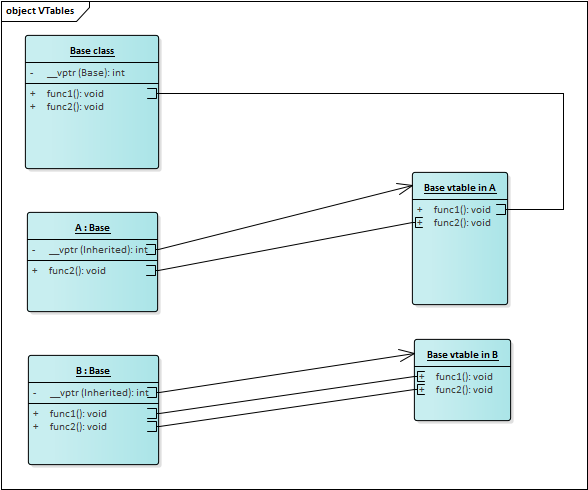
\includegraphics[scale=0.50]{./imgs/vtables.png}
\end{center}

In a base class with at least one virtual function is there, the virtual table constructed, and as you can see from the previous figure, in the base class a virtual point \textit{\_\_vptr} is used to point of this virtual table \textit{vtable} for each class will inherit from the base, and you might noticed that the virtual table is just an array of pointer to functions which will refer to a certain function in the base or in the Derived class.\\
if the Derived class is inheriting for the Base, and then the Derived is overriding this feature of the Base, this is called a Polymorphism which we have features are already inherited with no change but there are others will be overridden by a new feature/properties/behaviors in the Derived classes, and this is also referring to a "Late Binding Concept", as in the runtime this binding is happened by the help of the virtual tables unlike the Early Binding by the complier for the overloaded functions at the compile time.\\

To understand more, let's have a real example and then to look at a memory layout of a Base and Derived classes:

\lstinputlisting[language=C++, caption=Changing the behavior of a Base class]{cpp_code/inheritance/virtual-object-layout.cpp}

And by using clang AST, we can explore the class layout dump as following:
\lstinputlisting[language=C++, caption=Derived Class layout]{cpp_code/inheritance/virtual-table-layout}


Please refer also to \href{https://shaharmike.com/cpp/vtable-part1/}{this} interesting article to do the same but using GDB.


\subsubsection{The use of virtual, override, and final specifiers}


With the override keyword; you will force the compiler to check the base class to see if there is a virtual function with this \textbf{exact signature}. And if there is not, the compiler will a compilation error.

Note:
The virtual keyword is not necessary in the derived class. However it makes code clearer. Also in C++11 override keyword is introduced which allows the source code to clearly specify that a member function is intended to override a base class method.

\subsubsection{The sub-objects layout}
Follow this links: \href{https://www.linuxtopia.org/online_books/programming_books/c++_practical_programming/c++_practical_programming_222.html}{Cpp Sub-Objects}

\subsection{Writing a template class}
You might need to implement a generic class, and a sake of organization you might also need to implement it in separate .hpp and .cpp files, if you faced some problems while doing that, we might go together to understand how it works.

\subsubsection{template template parameters}

\subsubsection{Variable template C++14}

\subsection{The Cpp Run-time Type Information (RTTI) Support}
RTTI stands for Run-Time Type Information. It is used to retrieve information about an object at runtime (as opposed to compile time). In non-polymorphic languages there is no need for this information, because the type is always known at compile time and so in runtime. In a polymorphic language like C++, there are situations where the concrete type is not known at compile time.\\

Normally you can achieve that by using:
\begin{itemize}
  \item \textit{typeid} operator
  \item and \textit{typeinfo} class 
\end{itemize}

\textit{typeid} returns \textit{const std::type\_info} which can be accessed to get the \textit{typeinfo::name}, \textit{typeinfo::hash\_code} C++ 11 only, and you need to note that in C++ "The copy and assignment operators of type\_info are deleted: objects of this type cannot be copied."\\
\lstinputlisting[language=C++, caption=RTTI using the typeid operator]{cpp_code/polymorphism/rtti.cpp}

Also you need to know that the comparison operators "==" and "!=" are overloaded in this class which means that you can use to compare between object types at runtime.
\lstinputlisting[language=C++, caption=references v.s. Pointers]{cpp_code/polymorphism/rtti-comparsion.cpp}

\subsection{Virtual inheritance}
In general there are different types of inheritance:
\begin{itemize}
  \item Single Inheritance
  \item Multiple Inheritance
  \item Hierarchical Inheritance
  \item Multi-level Inheritance
  \item Hybrid (Virtual) Inheritance
\end{itemize}

We  will discuss here an issue with the virtual inheritance, and the Diamond Problem in the hybrid inheritance.
As you can see in the figure below, the hybrid inheritance might consist of different kinds of inheritance, let's say \textbf{Multiple Inheritance} as per "D" inherits from both "B" and "C", and \textbf{Hierarchical Inheritance} as "B" and "C" inherits from "A", and \textbf{Multilevel Inheritance} as "D" inherits from "B" or "C" and both inherits from "A (This forms a diamond!).\\

The problem here, as "A" class has a member function called \textit{foo()}, then it will be inherited in both "B" and "C", the both will be having this function, when "D" tries to inherit from both, then which \textit{foo()} function will be there !.\\
\begin{center}
  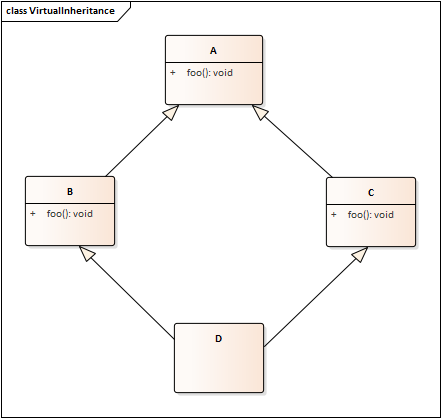
\includegraphics[scale=0.75]{./imgs/VirtualInheritance.png}
\end{center}

To be honest, the complier will throw an error: Ambiguous Type!
\lstinputlisting[language=C++, caption=The Virtual Inheritance Problem]{cpp_code/inheritance/virtual-inheritance-problem.cpp}

\begin{center}
  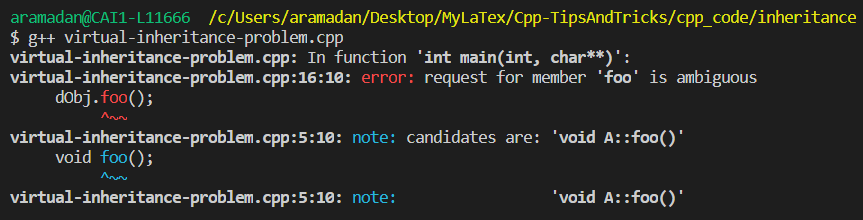
\includegraphics[scale=0.75]{./imgs/vinheritance-problem.PNG}
\end{center}

but after we defined the inheritance of "B" and "C" to "A" as virtual, then it's been solved and you can compile normally!.
\lstinputlisting[language=C++, caption=The Virtual Inheritance Solution]{cpp_code/inheritance/virtual-inheritance-solution.cpp}


\begin{center}
  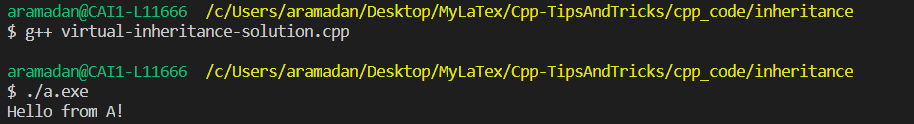
\includegraphics[scale=0.75]{./imgs/vinheritance-solution.PNG}
\end{center}

When a base class is specified as a virtual base, it can act as an indirect base more than once without duplication of its data members. A single copy of its data members is shared by all the base classes that use virtual base.

\subsection{Dynamic Dispatch and late binding (Polymorphism)}
In C++ the Polymorphism can be achieved in two ways: 
\begin{itemize}
  \item Compile time Polymorphism (Function Overloading)
  \item Runtime Polymorphism (Late Binding)
\end{itemize}

\section{Advanced Topics}
\subsection{Lambda Expression}
The lambda expression, anonymous functions or inline function pointers are used in the code were a complete function prototype is not needed and the function will be used only in this location.\\
You can define a lambda expression as follow:\\
\lstinputlisting[language=C++, caption=Using Lambda Expression Notation]{cpp_code/new_features/define-lambda-cpp}

As a simple usage of inline lambda expression:
\lstinputlisting[language=C++, caption=Using Lambda Expression Example]{cpp_code/new_features/lambda-expression01}

You can use lambda expression to define a behavior of STL algorithm 
\lstinputlisting[language=C++, caption=Use lambda expression to define a STL algorithm behaviour]{cpp_code/new_features/lambda-expression02}

\subsubsection{Using the STL algorithms}
The following code example used count\_if() with defined lambda expression, the function defines a count if greater than 5:
\lstinputlisting[language=C++, caption=C++ Example]{cpp_code/tempates.cpp}

\subsection{The C++ Casting Techniques}
Along with the C-Style casting, the C++ offers some other four casting techniques. you can use these techniques to cast from two in-comparable types if needed:
\begin{itemize}
  \item static\_cast<T>()
    
  if you tried to cast from float to int, your compiler might promote a warning to you that you will loss precision. but if you need to make this cast happen, you might think of using the static cast to cast between two in-completable types.

    \lstinputlisting[language=C++, caption=Static Cast example]{cpp_code/cpp-casting/static_cast.cpp}

  \item const\_cast<T>()
  if you tried to modify a constant value intentionally, the your complier will throw a compilation error that this is a wrong conversion operation.

  \begin{center}
    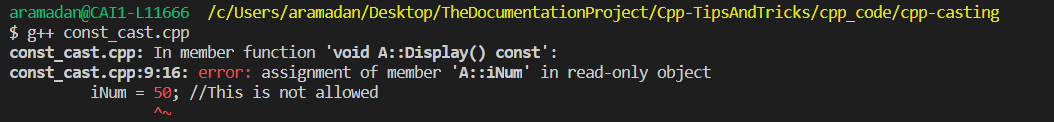
\includegraphics[scale=0.50]{./imgs/cpp_casting/const_cast.PNG}
  \end{center}

    You can use a const\_cast() to force the conversion from a const types to mutable type.
    \lstinputlisting[language=C++, caption=const cast]{cpp_code/cpp-casting/const_cast.cpp}


  \item reinterpret\_cast<T>()
    If you tried to cast one pointer type to another, the compiler might not allow that, but you can force that using the reinterpret cast.

    \begin{center}
      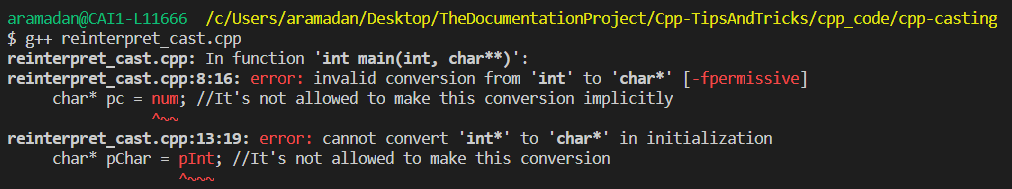
\includegraphics[scale=0.50]{./imgs/cpp_casting/reinterpret_cast.PNG}
    \end{center}

    reinterpret cast is a powerful casting method, it can cast between any two types, it's mainly used to convert between pointers types (be careful when you use it).

    \lstinputlisting[language=C++, caption=reinterpret cast]{cpp_code/cpp-casting/reinterpret_cast.cpp}

  \item dynamic\_cast<T>()
  You might use the dynamic cast in the down-casting, as by default you can't cast pointer of Derived class to pointer of a base class, so the dynamic cast is used to achieve that. 

  \lstinputlisting[language=C++, caption=Dynamic Cast]{cpp_code/cpp-casting/dynamic_cast.cpp}

  Compiling the above code without dynamic cast, the complier will throw an error.
  \begin{center}
    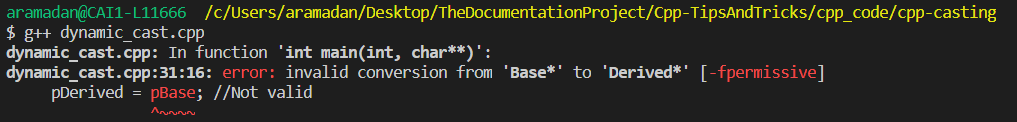
\includegraphics[scale=0.50]{./imgs/cpp_casting/dynamic_cast_downcasting.PNG}
  \end{center}
\end{itemize}

\begin{mybox}[title={Upcasting V.s. Downcasting}]
  By default in C++, the upcasting is allowed, as you can assign a "Derived" class pointer to a "Base" class pointer, but the Down-casting is not allowed as you can't assign a "Base" class pointer to a "Derived" class pointer, but you need to notice that you can achieve a down-casting using the C++ \textit{dynamic\_casting<T>()} technique.
\end{mybox}

\subsection{Cpp Perfect forwarding and universal references}

\subsection{decltype specifier}
\subsubsection{decltype, what is new in C++14}

\subsection{using keyword, using-declaration and type aliasing}

\subsubsection{type aliasing with "sing V.s. typedef}

\subsection{The Smart Pointers (C++11)}
What are smart pointer ?\\
It's a wrapper around the normal C++ pointers by using a template classes that uses operator overloads to provide a pointer functionality and provide a way more better for memory management. 
For example:
this function returns a pointer, but I have no idea after using this pointer what to do, which might cause a memory leaks.
T * foo();\\\\

but by using this for example: unique\_pointer<T> foo();\\
You know now that we should have only one copy of the this pointer, then after we finish with it, either to destroy it or to change its ownership.

\subsection{Cpp Async Programming, futures and promises}

\subsubsection{Types of Smart Pointers}
\begin{itemize} 
  \item Unique pointer: unique\_pointer<T> foo();
    Only one copy of the pointer should be there, and it will be released automatically if it's no longer used.

  \item Shared Pointer: shared\_pointer<T> foo();
    We might have multiple copies of the pointer, and it will be all released after all the copies no longer used.
  
  \item Weak Pointer: is a special kind of the shared pointers, and it used when you need avoid a circular references (objects depends on others so you can't destroy one before destroying the other one and vice versa).
\end{itemize}

Note: In order to use the smart pointers, you need to include the memory.h header file \textit{\#include<memory>}

\subsubsection{Unique Pointers}
It can't be copied, there is only one copy of the pointer. and need to use the unique\_pointer if a resources is only available to only one object at a time.

\lstinputlisting[language=C++, caption=Unique Pointers]{cpp_code/tempates.cpp}


\begin{itemize}
  \item unique\_pointer::move() function
  \item unique\_pointer::reset() function
  \item unique\_pointer::release() function
  \item make\_unique<>() function (non std)
\end{itemize}

Note: You can't pass a unique\_pointer to a function, because it's unique which can't be copied, so don't pass it by value, instead pass it by reference.


\subsubsection{Shared Pointer}
In the shared pointers, you may taking copies of the pointer. and the shared pointer class will keep a counter of the copies by using the shared pointer constructors and destructors.

The counter is called the reference count and can be accessed using \textit{shared\_pointer.use\_count()} function.

\subsubsection{Custom Deleters}
You can specify a custom deleter to be called with smart pointer reset function.

\subsection{Move Semantics (C++ 11)}
In move semantics, we move an object by re-associate it to a new object instead of copying it. suppose the following

\textit{T f(T o) { return o; }\\
        T b = f(b);
}\\
so here in the previous example, the object's copy constructor will be called twice on at the function call, and other one at the return type which creates a temporary not used object to be destructed later and this might consume an amount of time and memory usage till the temporary object is deleted.

Moving the data is taken place by using something called \textbf{\textit{rvalue reference}}, and you need to notice that it's different from the normal reference types which is called \textbf{\textit{lvalue reference}} 
\begin{itemize}
  \item T \& x    - lvalue reference (can't be moved as it's in left side of an assignment operator!)
  \item T \&\& x  - rvalue reference (can be moved)
\end{itemize}

\lstinputlisting[language=C++, caption=Using move semantics]{cpp_code/new_features/move-semantics01}
\textbf{Output}:\\
\begin{center}
  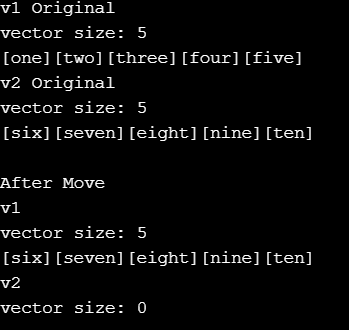
\includegraphics[scale=0.75]{./cpp_code/new_features/move-semantics01.PNG}
\end{center}

\subsubsection{Creating Move Constructors}

\subsubsection{Creating Move Assignment Operator}

\end{document}